\documentclass[11pt,oneside]{book}

\usepackage[T1]{fontenc}
\usepackage[french]{babel}

\usepackage[utf8]{inputenc}
\usepackage{graphicx}
\usepackage{grffile}
\usepackage{longtable}
\usepackage{wrapfig}
\usepackage{rotating}
\usepackage[normalem]{ulem}
\usepackage{amsmath}
\usepackage{textcomp}
\usepackage{amssymb}
\usepackage{capt-of}
\usepackage[colorlinks=true,linkcolor=black,citecolor=black]{hyperref}
\usepackage{textgreek}
\usepackage{minted}
\usepackage{framed}
\usepackage{mdframed}
\usepackage{geometry}
\usepackage{titlesec}
\usepackage{pdfpages}
\usepackage[textwidth=16mm]{todonotes}

\newcommand{\as}[1]{\todo[color=green!40,size=\tiny,caption={}]{#1}}
\newcommand{\asi}[1]{\todo[inline,caption={},color=green!40]{#1}}

\geometry{
a4paper,
left=18mm,
right=18mm,
top=20mm,
bottom=20mm
}

\begin{document}

\includepdf[pages=-]{page1.pdf}

\pagestyle{empty}
\fontfamily{cmss}
\selectfont

\setlength{\parindent}{4mm}

\setcounter{tocdepth}{1}
\tableofcontents
\pagenumbering{gobble}

\chapter{Introduction}
\pagenumbering{arabic}
\setcounter{page}{1}
\pagestyle{fancy}
\fancyhf{}
\cfoot[\thepage]{\thepage}

Ce projet nous a été proposé par l’équipe \href{https://www-intuidoc.irisa.fr/}{IntuiDoc}
de l’\href{https://www.irisa.fr/}{IRISA}, en étroite collaboration avec la startup
\href{http://www.doptim.eu}{Doptim} et avec le soutien de Jean-Yves LE CLERC, conservateur du
patrimoine aux \href{http://archives.ille-et-vilaine.fr/fr}{archives départementales} d'Ille-et-Vilaine.
Tout au long de l’année, nous serons encadrés par Bertrand COÜASNON, enseignant-chercheur membre d'IntuiDoc,
Erwan FOUCHÉ, chef de projet chez \href{https://www.soprasteria.com/fr}{Sopra Steria}, Julien BOUVET,
ingénieur chez Sopra Steria également. Nous serons aussi accompagnés par Sophie TARDIVEL, responsable
et \textit{data scientist} chez Doptim.

\paragraph{}
Ce projet a pour but de fournir un programme permettant de concevoir des bases d’apprentissage
automatiquement pour l’entraînement de divers systèmes de reconnaissance d’écriture manuscrite,
ainsi que leur exploitation, une base d'apprentissage étant un ensemble
d'exemples sur lesquels les reconnaisseurs vont pouvoir s'entraîner à associer
du texte de documents manuscrits ou imprimés à une transcription. Ces reconnaisseurs seront, par exemple,
capables de retranscrire de manière informatique des documents manuscrits
(registres paroissiaux, registres d’état civil, documents d’entreprise,
\ldots) pour les rendre plus exploitables. Ce projet permettra donc de gagner
du temps sur la compréhension de documents anciens en rendant l’entraînement
de systèmes complexes plus simple.

\paragraph{}
Ce projet est en lien avec les archives départementales d’Ille-et-Vilaine dans le cadre de la transcription numérique de registres paroissiaux et autres documents anciens. La sauvegarde et 
l’accès à ces documents est un enjeu important et notre projet consiste en un premier pas pour 
résoudre ce défi. Le rapport de pré-étude présente un aspect plus détaillé du contexte et des enjeux.

\paragraph{}
Dans ce rapport, nous définirons premièrement les spécifications générales du
projet, ainsi que celles de ses éléments. Nous détaillerons donc les
spécifications concernant la préparation des données en entrée, le stockage
des données, les liens avec un système de reconnaissance
d’écriture manuscrite, et enfin l’interface utilisateur. Nous expliquerons
ensuite l’architecture logicielle du projet, la façon dont les éléments
précédemment cités seront construits et liés ensemble. Enfin, nous conclurons
en abordant la suite du projet.

\paragraph{}
Le vocabulaire utile à la compréhension de ce rapport, déjà défini dans le
rapport de pré-étude, est rappelé en annexe 1.


\chapter{Cahier des charges}

Dans cette partie nous allons détailler les différentes caractéristiques
de notre projet. Nous allons commencer par étudier les différents objectifs
du projet puis nous l’analyserons plus en détail aux moyens d’outils de spécification.

\section{Les objectifs}

Les différents objectifs sont illustrés par le schéma en fin de section. Celui-ci,
bien que complexe, peut aider le lecteur à comprendre les liens entre tous les objectifs.
Les éléments \textbf{en gras} nous sont fournis et sont à intégrer dans le projet.

\paragraph{}
Le premier objectif est de découper correctement les documents manuscrits sous la forme
d’imagettes qui contiennent seulement une ligne du document à l’aide d’un
\textbf{outil de détection de lignes}. Cette partie correspond à la zone du schéma sur fond bleu.
Le \textit{scan} d’un document contenant des informations manuscrites est donné en entrée et est découpé en paragraphes
grâce aux \textbf{données de position} présentes dans les fichiers de la \textbf{base Maurdor}. Ces
paragraphes sont par la suite découpés en lignes via l’outil détecteur de lignes. Les éléments obtenus
sont enfin convertis en imagettes avec un programme à créer appelé \textit{Génération d’images} sur le schéma.

\paragraph{}
Le deuxième objectif est de relier les imagettes à leur retranscription numérique
(aussi appelée vérité terrain). Cet objectif est réalisable grâce aux données de position
qui accompagnent les retranscriptions de la base Maurdor. Ces couples \texttt{(imagette, retranscription)}
seront ensuite enregistrés dans une base de données qui constituera la base d’apprentissage du
système de reconnaissance d’écriture manuscrite. Cette partie correspond également à la partie
en bleu du schéma. Une vérité terrain permet non seulement d’identifier les paragraphes mais
également de lier les imagettes à la retranscription numérique du texte manuscrit qu’elles contiennent
grâce aux informations de numéro de ligne. Les imagettes (ou lignes sur le schéma) sont stockées
dans la base de données, en jaune. La base de données contient donc des imagettes (\textit{Exemples d’apprentissage}),
pouvant être associées à leur retranscription numérique (\textit{Label}) et à un texte généré par un
reconnaisseur d’écriture manuscrite (\textit{Résultats}).

\paragraph{}
Le troisième objectif est de générer les couples \texttt{(imagette, retranscription)} avec un format spécifique
qui pourra ensuite être facilement modifié, cela dans le but d’être compatible avec les formats d’entrée de
plusieurs systèmes de reconnaissance d’écriture manuscrite sans trop d’efforts.
Plusieurs choix s’offrent à nous. Comme les données en entrée sont dans le
\href{https://lampsrv02.umiacs.umd.edu/projdb/project.php?id=53}{format GEDI}, nous pourrions générer des
fichiers dans ce même format. Nous pouvons également les sauvegarder au format PiFF\cite{piff:2017},
fortement compatible avec ce type de données. Dans tous les cas, nous devrons créer un script qui
convertira les données (GEDI ou PiFF) en un format compatible avec le logiciel de reconnaissance d’écriture
manuscrite en notre possession. Le passage par le format GEDI ou PiFF permettra simplement de rendre les données
plus manipulables pour des personnes souhaitant les exploiter. Le système de reconnaissance d’écriture manuscrite
est situé dans la partie verte du schéma. Il devra posséder deux modes de fonctionnement :

\begin{itemize}
\item un mode d’\textbf{apprentissage} : dans ce mode, le système de reconnaissance extrait de la base de données les
imagettes et leur label associé pour pouvoir s'entraîner; il fournit ensuite un résultat pour chaque imagette,
qui pourra être comparé par des utilisateurs via une IHM;
\item un mode de \textbf{production} : dans ce mode, le reconnaisseur est censé être bien entraîné; il n’a que les
imagettes en entrée et il fournit une retranscription numérique (un label) pour des documents sans vérité terrain.
\end{itemize}

\paragraph{}
Le quatrième objectif est de créer une Interface Homme-Machine (IHM) permettant d’observer les imagettes
et les retranscriptions, afin de confirmer et/ou corriger les retranscriptions si jamais elles ne correspondent
pas au texte de l’imagette. On doit également pouvoir supprimer des couples \texttt{(imagette, retranscription)}
de la base de données si jamais l’utilisateur considère qu’elles n’apporteront rien de bénéfique
à l’apprentissage du reconnaisseur. Les données que l'on pourrait vouloir supprimer seraient des
données trop bruitées, trop dégradées, mal coupées, etc. Il pourrait cependant être intéressant
de les conserver pour que le reconnaisseur apprenne à reconnaître des textes abîmés. Cet objectif est représenté
dans la partie rouge du schéma, l'IHM locale, qui doit pouvoir accéder à la base de données et la modifier.

\paragraph{}
Enfin, le dernier objectif (optionnel) est de créer une seconde interface permettant
d’observer les imagettes et les résultats du reconnaisseur. Cet objectif est optionnel
car il sort légèrement du cadre du travail qui nous est demandé mais il sera utile pour faire
une démonstration du reconnaisseur lors de la présentation finale de notre projet.
Nous pourrons ainsi montrer ce que notre travail aura pu apporter à la reconnaissance
d’écriture manuscrite. Cette tâche ne sera probablement pas longue à réaliser car elle peut
consister en une amélioration de l’IHM précédente. Pour rendre la démonstration plus
ludique, on pourrait aussi imaginer créer une IHM sous forme de jeu entre une personne
et le reconnaisseur. Par exemple, la personne et le reconnaisseur pourraient avoir à
retranscrire un texte manuscrit le plus vite possible. Cet objectif est représenté dans
la partie rouge du schéma, l'IHM web, qui doit comme la première interface
accéder à la base de données et la modifier.

\paragraph{}
\begin{mdframed}[frametitle={Schéma représentant les différents objectifs du projet}, innerbottommargin=10]
\begin{center}
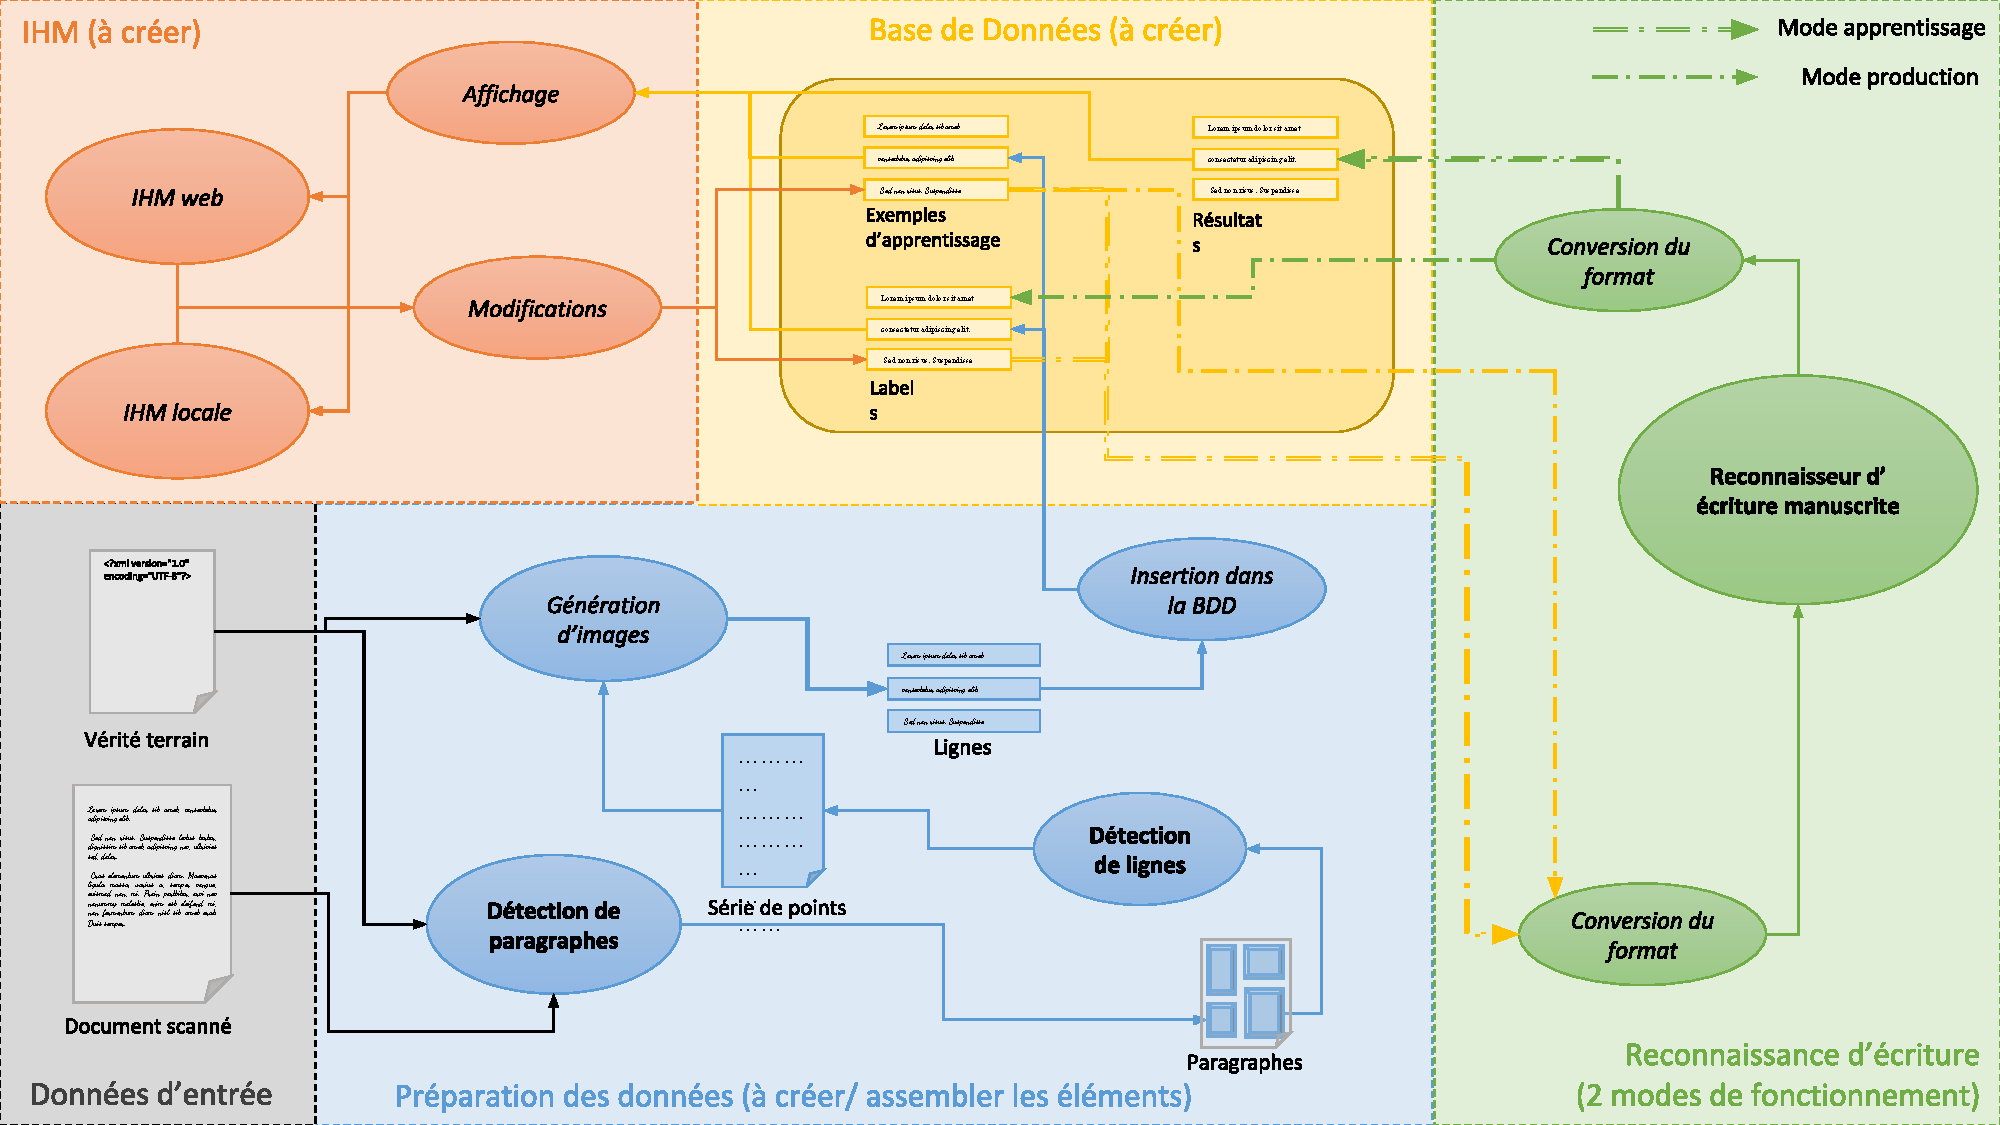
\includegraphics[width=\linewidth]{schema.pdf}
\end{center}
\end{mdframed}

\newpage
\section{Description fonctionnelle des besoins}

\subsection{Diagramme bête à cornes}

Le diagramme suivant permet d’exprimer le besoin lié au projet. Ainsi, notre logiciel de
traitement de données manuscrites aura pour but principal de préparer et stocker des données
d’apprentissage pour le système de reconnaissance d’écriture manuscrite développé par Doptim.

\paragraph{}
\begin{mdframed}
\begin{center}
\includegraphics[width=0.7\linewidth]{bete-a-cornes.png}
\end{center}
\end{mdframed}

\subsection{Diagramme pieuvre}

Le diagramme pieuvre, quant à lui, permet d’exprimer les différentes fonctions contraintes
qui découlent de l’objectif principal du projet. De ce fait, notre logiciel devra interagir
avec différents acteurs afin de s’intégrer parfaitement dans l’optique du projet :

\begin{itemize}
\item \textbf{FP1} : Tout d’abord, le premier objectif (et l’objectif principal du projet) est
de préparer et stocker les données d’apprentissage pour un système de reconnaissance d’écriture manuscrite.
\item \textbf{FC1} : Ensuite, il devra utiliser le détecteur de lignes fourni afin de découper
les phrases des textes d’entrée en imagettes. 
\item \textbf{FC2} : Il devra également permettre à l’utilisateur d’interagir avec les données
traitées afin de les vérifier et/ou de les modifier si nécessaire, le tout par le biais d’une Interface Homme-Machine. 
\item \textbf{FC3} : Notre logiciel utilisera aussi la vérité terrain fournie afin d’associer
les imagettes découpées à la bonne transcription.
\item \textbf{FC4} : Il faudra également que celui-ci soit compatible avec le format des données
qui lui seront fournies en entrée (format GEDI ou PiFF).
\item \textbf{FC5} : Enfin, notre logiciel devra regrouper les données afin de les stocker dans une base de données.
\end{itemize}

\paragraph{}
\begin{mdframed}
\begin{center}
\includegraphics[width=0.7\linewidth]{pieuvre.png}
\end{center}
\end{mdframed}

\newpage
    
\chapter{Contexte du projet}

Comme énoncé dans l’introduction, ce projet est en collaboration avec l’entreprise
Doptim et les archives départementales d’Ille-et-Vilaine. Le produit de notre travail
leur sera donc mis à disposition afin qu’ils puissent l’exploiter.

\section{Les archives départementales d’Ille-et-Vilaine}

Les archives départementales d’Ille-et-Vilaine, situées à Rennes, regroupent plusieurs
millions de documents manuscrits datant, pour les plus anciens, du début du XI\up{ème} siècle.
Ces documents n’y sont pas seulement entreposés mais aussi numérisés pour que n’importe qui
puisse les consulter, soit en version physique aux archives, soit en version numérique
depuis n’importe où. Il existe actuellement des moteurs de recherche permettant de retrouver
les documents grâce à des annotations ou des mots-clés, mais leur utilisation reste limitée
car les documents sont souvent peu lisibles. L'outil que notre projet va apporter aux
archivistes leur permettra de retranscrire la totalité du contenu d’un document manuscrit
sous forme de texte numérique pour que la recherche soit plus efficace et la consultation
plus agréable. Cet outil pourra facilement être intégré à la chaîne d’archivage des documents
puisqu’il pourra être exécuté juste après la numérisation, sans grande intervention humaine.

\section{Doptim}

Doptim est une entreprise spécialisée dans le \textit{Big Data} et l’analyse de données.
Elle a été fondée par Sophie TARDIVEL, qui sera notre contact dans l’entreprise.
Son but premier est de créer une communauté de \textit{data scientists} et de
\textit{data engineers} qui auraient l’ambition d’optimiser et de maîtriser la gestion
des données. Doptim est aujourd’hui investie dans un projet de service en ligne permettant
aux généalogistes de gagner du temps dans la fouille et le décryptage de documents numériques.
Notre projet pourrait donc être ajouté au leur pour simplifier la lecture de documents anciens.

\paragraph{}
Bien sûr, l’outil final de notre projet qui a pour but d’être compatible avec plusieurs
types de reconnaisseurs d’écriture manuscrite ne sera pas notre propriété. Nous le rendrons
public et utilisable par qui le veut. La collaboration que nous avons avec les archives
départementales d’Ille-et-Vilaine et Doptim nous permettent d’orienter notre projet afin de
nous faire une idée de ce qu’un utilisateur pourrait en attendre (notamment au niveau de l’IHM).
Ces deux collaborations ne sont pas distinctes puisque Doptim et les archives travaillent déjà ensemble.

\chapter{État de l'art}

Dans cette section, nous allons détailler tous les outils à notre disposition ainsi que leur fonctionnement.

\section{Techniques de reconnaissance d’écriture}

La plupart des techniques de reconnaissance de l’écriture sont basées sur des classifieurs
dits dynamiques, c’est-à-dire qu’ils possèdent une mémoire interne ou possèdent une notion
de contexte dans leur analyse. Ces classifieurs permettent un parcours et une division des
données d’entrées et donc d’effectuer une classification pour chacune des divisions repérées. 
		
\subsection{Modèles de Markov Cachés}

\subsection{Champs Aléatoires Conditionnels}

\subsection{Réseaux de Neurones Récurrents}

\section{Détecteur de lignes}

\subsection{Par floutage}

\subsection{Par réseau de neurone à convolution}

\section{Format de description d’image}

\subsection{GEDI}

GEDI est un outil qui permet d’annoter des documents scannés. Il est ainsi très utile pour établir
la vérité terrain. Il met en scène deux types de documents : des images qui correspondent aux documents
scannés ainsi que des documents XML au format GEDI qui permettent de stocker toutes les informations
relatives aux documents scannés. On peut alors avoir, pour chaque document scanné, des informations
relatives à la position des paragraphes, à la langue dans laquelle le texte est écrit, ou encore à
la forme du texte (manuscrit ou imprimé). La vérité terrain que nous aurons au sein de notre projet
aura été établie avec GEDI.

\subsection{PiFF}

Le Pivot File Format (PiFF) est un format de description d’image basé sur JSON et créé par différents
chercheurs français, dont notre encadrant de projet, Bertrand COÜASNON. Ce format est très utile pour l’analyse
de documents puisqu'il permet le partage de jeu de données, le traitement de résultats ainsi que
l’utilisation d’outils déjà existants sans avoir à faire de conversion entre les différents formats
qui pourraient exister. De ce fait, les différentes étapes de l’analyse de documents peuvent être effectuées
par différentes équipes sans qu’il n'y ait de conflit au niveau du format des données, ce qui permet une
collaboration plus facile. Les données présentes en entrée dans le cas de notre projet seront au format PiFF.
Par conséquent, les données après traitement par le logiciel devront également être dans ce format.

\chapter{Organisation du projet}

\section{Méthodes de travail}

Cette année, nous avons décidé d’utiliser une méthode de travail agile qui nous
semble la plus adaptée pour notre cas. En effet, nous allons commencer le développement
assez vite, pour voir ce qui est bien et ce qui n’est pas bien, pour pouvoir faire des
améliorations de manière continue. Ainsi, nous allons mettre en place des réunions
régulières pour voir l’avancée de la programmation.

\paragraph{}
Comme le projet peut facilement être découpé en 4 parties (Préparation des données,
Base de données, IHM et Gestion du reconnaisseur), nous avons décidé de diviser notre
groupe en 4 pour pouvoir faire avancer le projet en parallèle. Nous estimons qu’il est
tout de même important de garder une forte communication et cohésion entre les différents
groupes, donc nous avons mis en place différents systèmes de communication. Pour gérer
l’organisation, nous utiliserons Trello et Microsoft Project. Pour le partage de fichiers,
notamment pour la rédaction des rapports, nous utiliserons Google Drive et Git.
Pour la gestion du code, nous utiliserons aussi Git. Enfin, pour communiquer, nous
utiliserons une conversation Messenger (qui servira à transmettre des informations de
manière rapide), un groupe Facebook (qui servira à publier la répartition des tâches et
les objectifs de chaque semaine de manière fixe et accessible) et probablement des salons
Discord qui permettront à chaque groupe de communiquer sans perturber les autres groupes.

\paragraph{}
Pour l’instant, nous avons décidé d’établir des réunions hebdomadaires (voire deux réunions
par semaine en cas de retard ou de livrables à rendre). Cette planification sera probablement
modifiée au second semestre lors du début du développement, car le groupe sera réduit de
moitié à cause des départs en mobilité.

\section{Répartition des tâches}

Afin de répondre aux besoins du projet, nous avons mis en place 3 rôles. Ces 3 rôles ne sont pas fixes,
ils peuvent être modifiés en cas de besoin. Le premier rôle est le chef de projet. Ce rôle n’est pas fixe,
il change régulièrement. Nous avons établit un calendrier précis qui donne l’indication de qui
est chef de projet à chaque instant. Voici les rotations prévues :

\paragraph{}
\begin{tabular}{ | l | l | l | }
\hline
{\textbf{Chef de projet}}   &   {\textbf{Début}}    &   {\textbf{Fin}}  \\ \hline
{Kevin Despoulains}         &   {17/09/2018}        &	{07/10/2018}    \\ \hline
{Gaël Gendron}              &   {08/10/2018}	    &	{28/10/2018}    \\ \hline
{Corentin Guilloux}         &   {05/11/2018}	    &	{30/11/2018}    \\ \hline
{Valentin Foucher}          &   {01/12/2018}	    &	{13/01/2019}    \\ \hline
{Enzo Crance}               &   {14/01/2019}	    &	{04/02/2019}    \\ \hline
{Charlotte Richard}         &   {05/02/2019}	    &	{10/03/2019}    \\ \hline
{Laure Du Mesnildot}        &   {11/03/2019}	    &	{05/04/2019}    \\ \hline
{Timothée Neitthoffer}      &	{23/04/2019}	    &	{10/05/2019}    \\ \hline
\end{tabular}
    
\paragraph{}
Certaines périodes peuvent paraître plus longues pour certains que pour d’autres à cause des vacances
scolaires mais globalement chacun sera chef de projet durant 3 à 4 semaines. Le rôle du chef de projet est
avant tout de s’assurer du bon déroulement du projet. Il doit organiser les réunions, répartir équitablement
les tâches, surveiller les délais et diriger les réunions. Il doit également faire le lien avec les
différents intervenants et contrôler ce qui est écrit dans les rapports. Le deuxième rôle est celui de
responsable temps qui devra s’assurer que tout le groupe note bien le temps passé sur le projet en envoyant
des rappels réguliers. Il devra également gérer le temps de parole lors des réunions. Pour le moment,
c’est Timothée Neitthoffer qui a été désigné responsable temps. La personne jouant ce rôle peut être
modifié sans problème au cours de l’année. Enfin, le dernier rôle est responsable qualité. Son but est de
contrôler la qualité du code réalisé. Au premier semestre c’est lui qui valide ou non les technos que les
autres membres du groupe peuvent lui suggérer en les étudiant. Au second semestre il devra contrôler le code.
Pour le moment, c’est Enzo Crance qui a été désigné responsable qualité. Les autres membres du groupe travaillent
davantage sur les tâches que le chef de projet leur a confié comme la rédaction des rapports, la
recherche d’information, le développement, etc.

\section{Estimation de la planification des tâches}

Pour avoir une première estimation du planning, nous avons construit un diagramme de Gantt. L’explication est donnée en dessous.


Estimation de la planification des tâches
% GANTT

\paragraph{}
Les éléments en bleu correspondent à la prise en main du projet depuis la compréhension et l’analyse du projet
à la rédaction du cahier des charges. Cette partie se fait essentiellement en début de projet. Les éléments en rouge
correspondent à la rédaction des différents livrables. Nous avons estimé que le début de rédaction d’un livrable
doit se faire dès le rendu du livrable précédent. Les éléments en orange correspondent aux différentes soutenances.
Les dates de début de préparation sont pour l’instant difficiles à définir, la taille des blocs est donc provisoire.
Les éléments en vert correspondent au développement. Comme on peut le voir, il y a plusieures parties du développement
qui se font en parallèle. Les durées de chaques parties sont prévisionnelles mais sont susceptibles d’être grandement modifiées.
Enfin, les parties en rose correspondent au projet en production. Ce seront les tests du reconnaisseur.
    
\chapter{Conclusion}

Dans le cadre de notre projet de 4\up{ème} année en Informatique, nous avons
pour objectif de conduire un projet de la rédaction du cahier des charges
jusqu’à sa mise en production. Dans ce rapport, nous avons dans un premier
temps revu les spécifications de notre projet, tant dans son fonctionnement
interne que dans son interface avec un utilisateur ou un reconnaisseur
d’écriture manuscrite.

\paragraph{}
Nous avons ensuite détaillé la communication entre chacune des parties de
notre projet en décrivant son architecture générale et détaillée. Notre but
étant de rendre une application fonctionnelle pour la fin de l’année, nous
avions établi une première estimation du temps que prendrait chaque tâche
au cours du premier rapport. Cette estimation a pu être corrigée et améliorée
lors de l’étude des spécifications. De plus, nous avons pu nous projeter plus
en avant en choisissant de développer et de commenter une première version du
programme avant le départ de certains membres de notre équipe. Cette première
version pourra être améliorée plus facilement par les membres restants.

\paragraph{}
Enfin, nous avons défini une organisation qui nous semble judicieuse par
rapport à la configuration du projet, celui-ci pouvant être découpé en blocs.


\newpage
\bibliography{main}
\bibliographystyle{plain}

%%%
%% Author: timot
%% 30/01/2019
%%

% Preamble
\documentclass[11pt]{article}

% Packages
\usepackage{amsmath}

% Document
\begin{document}



\end{document}

\end{document}